\section{Distributed Graph Databases}
\label{sec:distr-graph-datab}

A distributed graph database employs a shared-nothing architecture, partitioning a graph among loosely cooperating servers.
Graph partitioning is non-trivial and a common approach is to use a $k$-balanced edge cut \cite{Huang2016}.
The objective of such an approach is to minimize the proportion of edges that span partitions and also to balance the distribution of vertices to partitions.
Fig \ref{dist-graph} depicts a graph database partitioned across 3 servers, $S_i, i = 1, 2$ and $3$.\footnote{Typically, each partition would be replicated for fault tolerance and availability, but these issues are beyond the scope of this paper.}

Intra-partition and inter-partition edges are respectively referred to as \textit{local edges}  and  \textit{distributed edges} (shown using dashed lines in Fig \ref{dist-graph}).
The proportion of distributed edges is not negligible and can range from 25-75\% \cite{Huang2016}.

\begin{figure}[ht]
  \centering
    \begin{tikzpicture}[node distance=1cm]

    \node (s1) [server,label=$S_1$] {};
    \node (s2) [server, right of=s1,xshift=1.5cm,yshift=1cm,label=$S_2$] {};
    \node (s3) [server, right of=s1,xshift=4cm,label=$S_3$] {};

    \node (v1) [vertex,xshift=-0.5cm,yshift=-0.8cm] {};
    \node (v2) [vertex, above of=v1,xshift=-0.1cm,yshift=0.7cm] {};
    \node (v3) [vertex, above of=v1,xshift=0.6cm] {};
    \node (v4) [vertex, below right of=v3,xshift=-0.5cm,yshift=-0.25cm] {};
    \node (v5) [vertex, above right of=v3,xshift=-0.1cm,yshift=-0.2cm] {};
    \node (v6) [vertex, right of=v5,xshift=0.5cm,yshift=0.8cm] {};
    \node (v7) [vertex, below of=v6, xshift=-0.15cm,yshift=0cm] {};
    \node (v8) [vertex, right of=v4, yshift=-0.1cm,xshift=4cm] {};
    \node (v9) [vertex, above of=v8,xshift=-0.4cm,yshift=-0.5cm] {};
    \node (v10) [vertex, above of=v9,xshift=-1.7cm,yshift=-0.33cm] {};
    \node (v11) [vertex, right of=v9,yshift=0.5cm,xshift=-0.3cm] {};
    \node (v12) [vertex, above of=v11,yshift=-0.3cm,xshift=-1cm] {};
    \node (v13) [vertex, above right of=v6,yshift=-0.4cm,xshift=-0.1cm] {};
    \draw [local] (v2) -- (v1);
    \draw [local] (v1) -- (v3);
    \draw [local] (v3) -- (v2);
    \draw [local] (v2) -- (v5);
    \draw [local] (v1) -- (v4);
    \draw [local] (v5) -- (v4);
    \draw [dist] (v5) -- (v6);
    \draw [dist] (v4) -- (v7);
    \draw [dist] (v8) -- (v4);
    \draw [local] (v8) -- (v9);
    \draw [local] (v9) -- (v11);
    \draw [local] (v10) -- (v7);
    \draw [dist] (v10) -- (v12);
    \draw [dist] (v12) -- (v13);
    \draw [local] (v10) -- (v6);
    \draw [dist] (v10) -- (v11);
    \draw [local] (v13) -- (v10);
    \draw [local] (v11) -- (v12);
    \end{tikzpicture}
  \caption{Local and distributed edges}
  \Description{Graph representation.}
  \label{dist-graph}
\end{figure}


Adjacency lists can now contain edge pointers to vertices on remote servers.
Guaranteeing reciprocal consistency for distributed edges is challenging, especially when an existing BASE database is used for storage and is then adapted with a query language expressed in terms of edges and vertices along with some gluecode to bind that interface to the underlying database.
Opting for this design appears to be a good choice: it offers the application programmer the modeling convenience of graphs together with the operational characteristics of the underlying BASE database.

However, a major problem with this design option is the lack of transactional semantics from the underlying BASE databases.
The latter seldom provide guarantees for multi-operation, multi-object transactions that span partitions. Without concurrency control across partitions, concurrent updates of distributed edges can interleave and violate reciprocal consistency.\footnote{The concurrency control primitives provided by BASE databases are typically sufficient to ensure reciprocal consistency for local edges.}
Our earlier work showed that undermining reciprocal consistency in distributed edges can lead to irreversible corruption of the distributed database itself and the corruption rate can be worryingly high (\cite{Ezhilchelvan2018}, \cite{Webber2019}).
Origins of reciprocal inconsistency in distributed edges are explained in Section \ref{sec:db-corruption}.

\begin{figure*}[ht]
  \centering
  \begin{subfigure}[b]{0.3\textwidth}
    \centering
    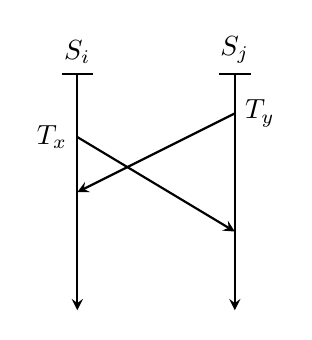
\begin{tikzpicture}
      \draw [thick] (1.3,3) -- (1.7,3);
      \draw [thick,<-,>=stealth] (1.5,0) -- (1.5,3) node[anchor=south] {$S_i$};
      \draw [thick] (3.3,3) -- (3.7,3);
      \draw [thick,<-,>=stealth] (3.5,0) -- (3.5,3) node[anchor=south] {$S_j$};
      \draw [thick,<-,>=stealth] (1.5,1.5) -- (3.5,2.5)  node[right] {$T_y$};
      \draw [thick,->,>=stealth] (1.5,2.2) node[left] {$T_x$} -- (3.5,1);
    \end{tikzpicture}
    \caption{}
    \label{fig:tx-ty}
  \end{subfigure}%
  \begin{subfigure}[b]{0.3\textwidth}
    \centering
    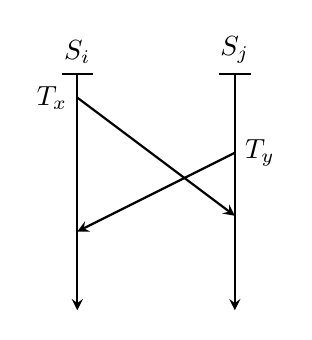
\begin{tikzpicture}
      \draw [thick] (5.3,3) -- (5.7,3);
      \draw [thick,<-,>=stealth] (5.5,0) -- (5.5,3) node[anchor=south] {$S_i$};
      \draw [thick] (7.3,3) -- (7.7,3);
      \draw [thick,<-,>=stealth] (7.5,0) -- (7.5,3) node[anchor=south] {$S_j$};
      \draw [thick,<-,>=stealth] (5.5,1) -- (7.5,2)  node[right] {$T_y$};
      \draw [thick,->,>=stealth] (5.5,2.7) node[left] {$T_x$} -- (7.5,1.2);
    \end{tikzpicture}
    \caption{}
\label{fig:ty-tx}
  \end{subfigure}%
  \begin{subfigure}[b]{0.3\textwidth}
    \centering
    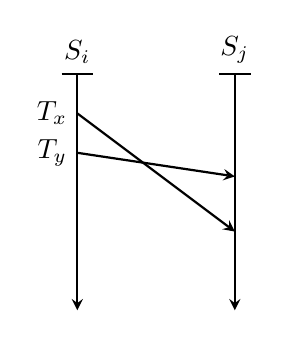
\begin{tikzpicture}
      \draw [thick] (9.3,3) -- (9.7,3);
      \draw [thick,<-,>=stealth] (9.5,0) -- (9.5,3) node[anchor=south] {$S_i$};
      \draw [thick] (11.3,3) -- (11.7,3);
      \draw [thick,<-,>=stealth] (11.5,0) -- (11.5,3) node[anchor=south] {$S_j$};
      \draw [thick,->,>=stealth] (9.5,2.5)  node[left] {$T_x$} -- (11.5,1) ;
      \draw [thick,->,>=stealth] (9.5,2) node[left] {$T_y$} -- (11.5,1.7);
    \end{tikzpicture}
    \caption{}
    \label{fig:same-side}
  \end{subfigure}%
  \caption{Possible interleavings of concurrent transaction's writes to a distributed edge spanning servers $S_i$ and $S_j$ by transactions $T_x$ and $T_y$. In \subref{fig:tx-ty} $T_y$ begins writing to the distributed edge before $T_x$, in \subref{fig:ty-tx} the converse is true, else they are equivalent. In \subref{fig:same-side} both transactions begin writing at the same server but overlap in the network and arrive out-of-order.}
  \label{conf-scen}
\end{figure*}
